\documentclass{article}%
\usepackage[T1]{fontenc}%
\usepackage[utf8]{inputenc}%
\usepackage{lmodern}%
\usepackage{textcomp}%
\usepackage{lastpage}%
\usepackage[head=40pt,margin=0.5in,bottom=0.6in]{geometry}%
\usepackage{graphicx}%
%
\title{\textbf{Fijan en Bs.S 800 mil crédito para compra de vivienda principal}}%
\author{BETSSY SATISTEVAN GASTELÚ}%
\date{26/11/2018}%
%
\begin{document}%
\normalsize%
\maketitle%
\textbf{URL: }%
http://www.eluniversal.com/economia/26688/fijan{-}en{-}bss{-}800{-}mil{-}credito{-}para{-}compra{-}de{-}vivienda{-}principal\newline%
%
\textbf{Periodico: }%
EU, %
ID: %
26688, %
Seccion: %
economia\newline%
%
\textbf{Palabras Claves: }%
NO\_TIENE\newline%
%
\textbf{Derecho: }%
2.8, %
Otros Derechos: %
, %
Sub Derechos: %
2.8.2\newline%
%
\textbf{EP: }%
NO\newline%
\newline%
%
\textbf{\textit{La medida fue publica en la Gaceta Oficial N° 41.525 del 15 de noviembre}}%
\newline%
\newline%
%
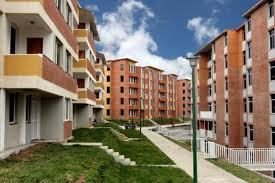
\includegraphics[width=300px]{218.jpg}%
\newline%
%
Caracas.{-} Hasta Bs.S 800.000,00 será el  crédito que otorgará el Ejecutivo Nacional para la adquisición de vivienda principal.\newline%
\newline%
En la Gaceta Oficial N° 41.525 de fecha 15 de noviembre de 2018, fue publicada la Resolución del Ministerio del para Hábitat y Vivienda mediante la cual se establecen las condiciones de financiamiento que regirán el otorgamiento de créditos para la adquisición, autoconstrucción, ampliación o mejoras de vivienda principal.\newline%
\newline%
Establece que para la autoconstrucción de vivienda principal el crédito será de hasta Bs.S 600.000,00.%
\newline%
%
El documento también impone que hasta Bs.S 450.000,00  será el financiamiento para  la ampliación de la vivienda principal.\newline%
\newline%
Determina que para mejoras de vivienda principal el préstamo será de hasta Bs.S  350.000,00.\newline%
\newline%
Los créditos para adquisición de vivienda principal podrán concederse por un plazo máximo de 35 años.\newline%
\newline%
En los casos de créditos para autoconstrucción de vivienda principal el plazo no excederá de 25 años.\newline%
\newline%
Para créditos destinados a la ampliación de vivienda principal el plazo no excederá de veinte (20) años y en los créditos de mejoras de vivienda principal el plazo no excederá de quince (15) años.%
\newline%
%
En el documento se ordena que los créditos para la adquisición, autoconstrucción, ampliación o mejoras de vivienda principal podrán ser otorgados hasta por el cien por ciento (100\%) del monto de la solicitud.\newline%
\newline%
Se crea el programa especial “Arma tu Crédito”, destinado a la adquisición de vivienda principal, el cual consiste en otorgar facilidades de financiamiento que mejore la capacidad de pago de la familia venezolana, mediante cuotas extraordinarias, variables y consecutivas, ajustables anualmente en función de los ingresos familiares.\newline%
\newline%
El programa especial “Arma tu Crédito”, será opcional para las familias venezolanas que así lo soliciten expresamente y sus condiciones particulares, serán regulados y establecidos a través de circular emitidas por el Banco Nacional de Vivienda y Hábitat.%
\newline%
%
\end{document}